\chapter{Problemas de filas}
\label{cap:filas}

Os sistemas de filas constituem importante classe de sistemas a eventos discretos (\acs{SED}s) em que entidades ou objetos devem esperar para obter um determinado recurso. Há três elementos básicos que compõem esses sistemas: \begin{itemize}
	\item consumidor: entidade que espera por um recurso;
	\item servidor: o recurso que é aguardado;
	\item fila: o espaço em que os consumidores esperam.
\end{itemize} Os recursos são genericamente denominados servidores por geralmente proverem serviço \cite{cassandras}. O presente trabalho aborda uma ótica abstrata dos sistemas de filas, já que há a possibilidade de reduzir problemas a estes sistemas.

Para ser atendido por um servidor de banco, uma pessoa deve esperar em uma fila até que as pessoas a sua frente sejam atendidas. Esse sistema de filas pode ser modelado pelo autômato infinito determinístico ilustrado pela figura \ref{fig:fila_simples_infinito}, em que $+$ e $-$ são os respectivos eventos de chegada e partida de pessoa da fila.

\figura{Um sistema de filas simples}{
	\begin{tikzpicture}[shorten >=1pt,node distance=2cm,on grid,auto] 
		\node[state,initial] (q0) {}; 
		\node[state] at (3,0) (q1) {};
		\node[state] at (6,0) (q2) {};
		\node[state,draw=none] at (9,0) (q3) {$...$};
		\draw
		(q0) edge[bend left, above] node{$+$} (q1)
		(q1) edge[bend left, below] node{$-$} (q0)
		(q1) edge[bend left, above] node{$+$} (q2)
		(q2) edge[bend left, below] node{$-$} (q1)
		(q2) edge[bend left, above] node{$+$} (q3)
		(q3) edge[bend left, below] node{$-$} (q2);
	\end{tikzpicture}
}{fig:fila_simples_infinito}{CASSANDRAS; LAFORTUNE, 1999}

Na figura \ref{fig:fila_simples_infinito} é assumido que a fila de pessoas pode crescer indefinidamente, o que não é possível na realidade. Assumindo que as filas têm um tamanho máximo, faz-se possível modelar os sistemas de filas por meio de autômatos finitos determinísticos (AFDs). Para muitos destes sistemas, além do mais, deseja-se que as filas respeitem uma capacidade máxima, sem que operações de adição sejam permitidas quando ela é alcançada. Outra propriedade frequentemente esperada é a de que nenhum evento de retirada seja possível quando há zero elementos na fila. A garantia de tais restrições é o que configura o problema do produtor-consumidor \cite{mehmood}, mas não se restringe a ele.

Um exemplo de sistema de filas é apresentado por \citeonline{victor} e consiste em uma planta de fila de demandas para veículos aéreos não tripulados (\acs{VANT}s). Nele as demandas são os consumidores, e os VANTs, os servidores. Seja o AFD da figura \ref{fig:demandas_vants}, em que os eventos $+$, $a$ e $-$ indicam a chegada, atribuição e conclusão de demanda. O modelo representa um sistema de fila de demandas para VANTs, cujas atribuições só podem ser retiradas da fila depois de concluídas e o tamanho da fila é no máximo $2$. O AFD torna-se complexo se consideramos a possibilidade de falhas e reatribuição, e determinar se restrições são atendidas fica ainda mais difícil.

\figuradoautor{Um sistema de demandas para VANTs}{
	\begin{tikzpicture}[shorten >=1pt,node distance=2cm,on grid,auto]
	\node[state,initial] (q0) {};
	\node[state] at (3, 0) (q1) {};
	\node[state] at (3, -3) (q2) {};
	\node[state] at (3, -6) (q3) {};
	\node[state] at (0, -6) (q4) {};
	\node[state] at (6, 0) (q5) {};
	\node[state] at (6, -3) (q6) {};
	\node[state] at (6, -6) (q7) {};
	\draw
	(q0) edge node{$+$} (q1)
	(q1) edge node{$+$} (q5)
	(q1) edge node{$a$} (q2)
	(q2) edge node{$-$} (q0)
	(q2) edge[left] node{$+$} (q3)
	(q3) edge node{$a$} (q4)
	(q4) edge node{$-$} (q2)
	(q3) edge node{$-$} (q5)
	(q5) edge node{$a$} (q6)
	(q6) edge node{$-$} (q1)
	(q6) edge node{$a$} (q7)
	(q7) edge node{$-$} (q2);
	\end{tikzpicture}
}{fig:demandas_vants} 

A julgar pela dificuldade de garantir consistências em SEDs, é eminente a relevância de métodos formais para inferências a respeito de propriedades dos AFDs. Antes de formular esses meios matemáticos, duas importantes propriedades dos sistemas de filas são expostas na próxima seção, \ref{sec:props}.

\section{Propriedades desejadas}
\label{sec:props}

Como citado para o problema do produtor-consumidor, um sistema de filas geralmente requer que duas propriedades inerentes sejam satisfeitas: que o tamanho máximo de cada fila não possa exceder uma capacidade máxima e não seja possível realizar operações de retirada em uma fila vazia. Isso decorre do fato de que normalmente as filas destes sistemas são representações de espaços físicos, com limitações que devem ser respeitadas nos modelos de SEDs.

O problema do produtor-consumidor decorre da necessidade de sincronizar um \textit{buffer} -- uma fila -- compartilhado entre processos. Na ciência da computação, a concorrência de processos sobre os mesmos recursos impõe que alguns artifícios de software e hardware sejam empregados a fim de respeitar as propriedades explanadas por esta seção. Sem eles, o desenvolvimento de aplicações computacionais com memória compartilhada gera defeitos que são manifestados no uso. Um exemplo deste problema é o caso em que dois processos tentam adicionar arquivo no \textit{spool} de impressão de um sistema operacional, o que, se não for sincronizado, possibilita a ambos os processos escreverem sobre a mesma célula do \textit{spool} \cite{tanenbaum}. No contexto da automação industrial, há também a necessidade de manter processos de produção e manufatura sincronizados. Máquinas que compartilham filas de recursos precisam atuar de modo consistente. 

Apesar de as representações de filas físicas requererem um volume mínimo de zero itens, esta pode não ser uma condição para filas abstratas. A subseção a seguir aborda esses e outros casos, em que é possível reduzir problemas abstraindo a noção de filas, servidores e consumidores.

\subsection{Redução de problemas}

É possível reduzir problemas à validação das propriedades supracitadas. Seja um SED com a seguinte restrição: há dois subconjuntos de eventos $E_1$ e $E_2$ tais que, em qualquer cadeia de eventos, o número de eventos pertencentes a $E_1$ menos o número de eventos pertencentes a $E_2$ deve ser menor ou igual a $n$. Abstraindo, podemos imaginar que um supervisor anota um símbolo em uma fila toda vez que um evento de $E_1$ é executado e apaga dela um símbolo quando um evento de $E_2$ é efetuado, da forma que a figura \ref{fig:reducao_fila} ilustra. Pode-se modelar esse SED como um sistema de filas em que os eventos de $E_1$ e $E_2$ sejam substituídos respectivamente por operações de adição e retirada de fila. Garantido que a fila tem capacidade máxima de $n$ itens, a restrição é satisfeita, porque, sempre que há $x$ símbolos na fila, foram executados $x$ eventos de $E_1$ a mais que de $E_2$.

\figuradoautor{Abstração de filas para redução de problemas}{
	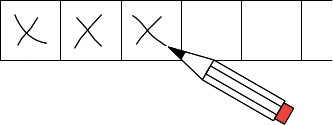
\includegraphics[width=.4 \textwidth]{figuras/reducao_fila.jpg}
}{fig:reducao_fila}

Há outros meios de reduzir problemas de SEDs à garantia das propriedades de sistemas de filas. Para tanto, deve-se encontrar meios de abstraí-los usando os conceitos que este capítulo apresentou. A exemplo dessas abstrações, seja o autômato da figura \ref{fig:exemplo_reducao1}, que descreve o funcionamento de uma linha de produção em que há uma esteira e dois robôs com sensores embutidos. Quando uma peça passa pela esteira e chega perto de um dos robôs, o sensor deste detecta a peça e emite sinal para que o robô pegue-a, faça algum trabalho nela e coloque-a em outra esteira. Se o primeiro robô está ocupado, o segundo detectará por seu sensor a peça passando e poderá executar o trabalho. Suponhamos que uma análise criteriosa do sistema foi levantada e originou o AFD ilustrado e identifiquemos os respectivos eventos $s_1$, $s_2$, $t_1$ e $t_2$ como a detecção de peça pelos sensores do primeiro e segundo robô e a execução de trabalho na peça pelo primeiro e segundo robô.

\figuradoautor{Autômato para o funcionamento de uma linha de produção simples}{
	\begin{tikzpicture}[shorten >=1pt,node distance=2cm,on grid,auto] 
	\node[state,initial] (q0) {}; 
	\node[state] at (3,0) (q1) {};
	\node[state] at (6,0) (q2) {};
	\node[state] at (9,0) (q3) {};
	\draw
	(q0) edge[bend left, above] node{$s_1$} (q1)
	(q1) edge[above] node{$t_1$} (q0)
	(q1) edge[above] node{$s_2$} (q2)
	(q2) edge[bend left, below] node{$t_2$} (q0)
	(q2) edge[above] node{$s_1$} (q3)
	(q3) edge[bend left, below] node{$t_1$, $s_2$} (q2)
	(q3) edge[bend right, above] node{$t_2$} (q1);
	\end{tikzpicture}
}{fig:exemplo_reducao1}

Sobre o sistema modelado pela figura \ref{fig:exemplo_reducao1}, utilizando a abstração por filas, podemos responder à pergunta: há uma carga máxima de trabalho que o segundo robô pode executar a mais que o primeiro? Seja, então, uma fila com todos os trabalhos que o segundo robô executa a mais que o primeiro. O sistema de filas da figura \ref{fig:exemplo_reducao2} apresenta tal redução, e notemos, pelo circuito destacado em vermelho, a existência de um ciclo que pode se repetir indefinidas vezes, adicionando um item à fila por vez. Isso evidencia uma característica da fila: não existe capacidade a limitando. Portanto, respondendo à pergunta, não há carga máxima relativa. O exemplo é simples, mas ilustra claramente uma redução de problema. Para problemas e SEDs complexos, esse procedimento mostra-se interessante, porque propicia o emprego dos métodos matemáticos do presente trabalho na resolução.

\figuradoautor{Autômato da figura \ref{fig:exemplo_reducao1} reduzido a um sistema de filas}{
	\begin{tikzpicture}[shorten >=1pt,node distance=2cm,on grid,auto] 
	\node[state,initial] (q0) {}; 
	\node[state] at (3,0) (q1) {};
	\node[state] at (6,0) (q2) {};
	\node[state] at (9,0) (q3) {};
	\draw
	(q0) edge[bend left, above] node{$s_1$} (q1)
	(q1) edge[above] node{$-$} (q0)
	(q1) edge[above,draw=red] node{$s_2$} (q2)
	(q2) edge[bend left, below] node{$+$} (q0)
	(q2) edge[above,draw=red] node{$s_1$} (q3)
	(q3) edge[bend left, below] node{$-$, $s_2$} (q2)
	(q3) edge[bend right, above,draw=red] node{$+$} (q1);
	\end{tikzpicture}
}{fig:exemplo_reducao2}

Especificadas as propriedades acima, resta-nos encontrar formalismos capazes de auxiliar a garantia delas. O capítulo seguinte, \ref{cap:propriedades}, propõe e exemplifica teoremas para esse propósito.

